\documentclass[tikz,border=6pt]{standalone}
\usepackage{amsmath,amssymb}
\usepackage{xcolor}
\definecolor{accent}{HTML}{A13D2C}
\definecolor{accent2}{HTML}{2B5F6B}
\definecolor{muted}{HTML}{5A564F}
\definecolor{panel}{HTML}{F8F6F0}
\definecolor{linecol}{HTML}{D8D2C4}
\definecolor{astroblue}{HTML}{1B4F72}
\usetikzlibrary{calc,arrows.meta,decorations.pathmorphing}
\usepackage[T1]{fontenc}\usepackage{newpxtext,newpxmath}  % same fonts as the notes
\begin{document}
% Schematic (not to scale) of an embedded protostar seen side on: dusty envelope, two outflow cavities,
% flattened disk, central protostar, bipolar jet and the bow shocks where the jet meets the cloud.
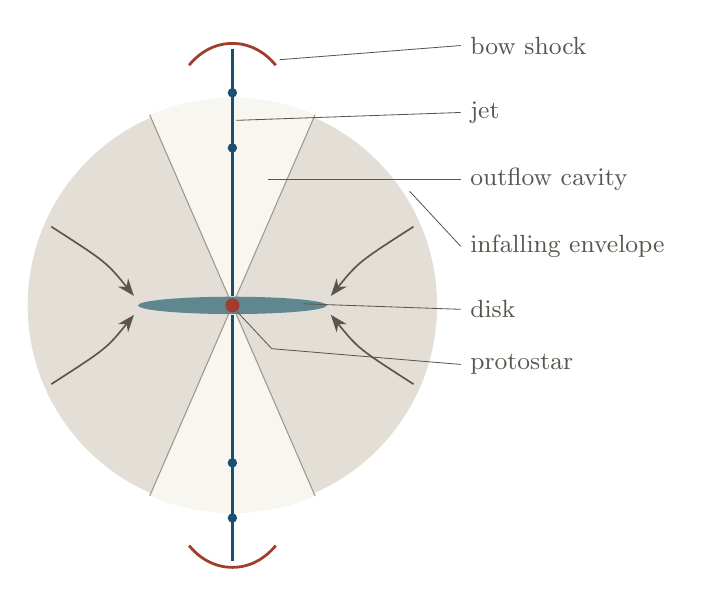
\begin{tikzpicture}[>={Stealth[length=2.2mm]}]
  % envelope
  \fill[linecol!70] (0,0) circle (2.6);
  % outflow cavities (cones about the axis)
  \fill[panel] (0,0) -- (-1.05,2.42) arc (113.5:66.5:2.64) -- cycle;
  \fill[panel] (0,0) -- (-1.05,-2.42) arc (246.5:293.5:2.64) -- cycle;
  \draw[muted!60, line width=0.4pt] (0,0) -- (-1.05,2.42) (0,0) -- (1.05,2.42)
                                    (0,0) -- (-1.05,-2.42) (0,0) -- (1.05,-2.42);
  % infall: curved streamlines from the envelope onto the disk
  \foreach \s in {1,-1} {
    \draw[->, muted, line width=0.6pt] (\s*2.3,1.0) .. controls (\s*1.6,0.55) .. (\s*1.25,0.12);
    \draw[->, muted, line width=0.6pt] (\s*2.3,-1.0) .. controls (\s*1.6,-0.55) .. (\s*1.25,-0.12);
  }
  % disk
  \fill[accent2!75] (0,0) ellipse (1.2 and 0.11);
  % protostar
  \fill[accent] (0,0) circle (0.09);
  % jet along the axis
  \draw[astroblue, line width=1.3pt] (0,0.12) -- (0,3.25);
  \draw[astroblue, line width=1.3pt] (0,-0.12) -- (0,-3.25);
  % knots and bow shocks
  \foreach \y in {2.0,2.7} { \fill[astroblue] (0,\y) circle (0.06); \fill[astroblue] (0,-\y) circle (0.06); }
  \draw[accent, line width=1.0pt] (-0.55,3.05) .. controls (-0.25,3.42) and (0.25,3.42) .. (0.55,3.05);
  \draw[accent, line width=1.0pt] (-0.55,-3.05) .. controls (-0.25,-3.42) and (0.25,-3.42) .. (0.55,-3.05);
  % labels with leader lines (right side)
  \draw[muted, line width=0.3pt] (0.6,3.12) -- (2.9,3.3) node[right, muted] {\small bow shock};
  \draw[muted, line width=0.3pt] (0.05,2.35) -- (2.9,2.45) node[right, muted] {\small jet};
  \draw[muted, line width=0.3pt] (0.45,1.6) -- (2.9,1.6) node[right, muted] {\small outflow cavity};
  \draw[muted, line width=0.3pt] (2.25,1.45) -- (2.9,0.75) node[right, muted] {\small infalling envelope};
  \draw[muted, line width=0.3pt] (0.9,0.02) -- (2.9,-0.05) node[right, muted] {\small disk};
  \draw[muted, line width=0.3pt] (0.06,-0.08) -- (0.5,-0.55) -- (2.9,-0.75) node[right, muted] {\small protostar};
\end{tikzpicture}
\end{document}
